\iffalse
\let\negmedspace\undefined
\let\negthickspace\undefined
\documentclass[journal,12pt,twocolumn]{IEEEtran}
\usepackage{cite}
\usepackage{amsmath,amssymb,amsfonts,amsthm}
\usepackage{algorithmic}
\usepackage{graphicx}
\usepackage{textcomp}
\usepackage{xcolor}
\usepackage{txfonts}
\usepackage{listings}
\usepackage{enumitem}
\usepackage{mathtools}
\usepackage{gensymb}
\usepackage[breaklinks=true]{hyperref}
\usepackage{tkz-euclide} % loads  TikZ and tkz-base
\usepackage{listings}
\usepackage{gvv}


\newtheorem{theorem}{Theorem}[section]
\newtheorem{problem}{Problem}
\newtheorem{proposition}{Proposition}[section]
\newtheorem{lemma}{Lemma}[section]
\newtheorem{corollary}[theorem]{Corollary}
\newtheorem{example}{Example}[section]
\newtheorem{definition}[problem]{Definition}

\newcommand{\BEQA}{\begin{eqnarray}}
\newcommand{\EEQA}{\end{eqnarray}}
\newcommand{\define}{\stackrel{\triangle}{=}}
\theoremstyle{remark}
\newtheorem{rem}{Remark}

\graphicspath{./figs/}

%\bibliographystyle{ieeetr}
\begin{document}
%

\bibliographystyle{IEEEtran}


\vspace{3cm}

\title{
	%	\logo{
	Assignment-2

	\large{EE:1205 Signals and Systems}

	Indian Institute of Technology, Hyderabad
	%	}
}
\author{Kunal Thorawade

EE23BTECH11035
}	

\maketitle


\newpage

%\tableofcontents

\bigskip
 
 \renewcommand{\thefigure}{\theenumi}
 \renewcommand{\thetable}{\arabic{table}}
 %\renewcommand{\theequation}{\theenumi}

 \section{Question:}
 What will Rs 500 amounts to in 10 years after its deposit in a bank which pays annual interest rate of 10$\%$ compounded annually?

 \section{Solution}
 \fi

 \begin{table}[ht]
	  \centering
	    \begin{tabular}{|c|c|c|}
		        \hline
			   \textbf{ Parameter} & \textbf{Value} & \textbf{Description} \\
			       \hline
			           $x(0)$ & 500 & Principal amount before first year \\
				       \hline
				           $r$ & 1.1 & Common ratio of GP \\
					       \hline
					           $n$ & 10 & Number of years   \\
						       \hline
						           $x(10)$ & $500(1.1)^{10} = 1296.87$ & Amount after 10 years  \\
							       \hline
							         \end{tabular}
								   \vspace{2mm}
								     \caption{Parameter Table}
								       \label{tab:11.9.3.31}
\end{table}


 The Z-transform of a sequence $x(n)$ is given by:

 \begin{align}
	     x(n) &= 500(1.1)^{n}u(n)
	       \\  X(Z) &= \frac{500}{1 - (1.1)z^{-1}} ; |z| > 1.1
 \end{align}

 \begin{figure}
	     \centering
	         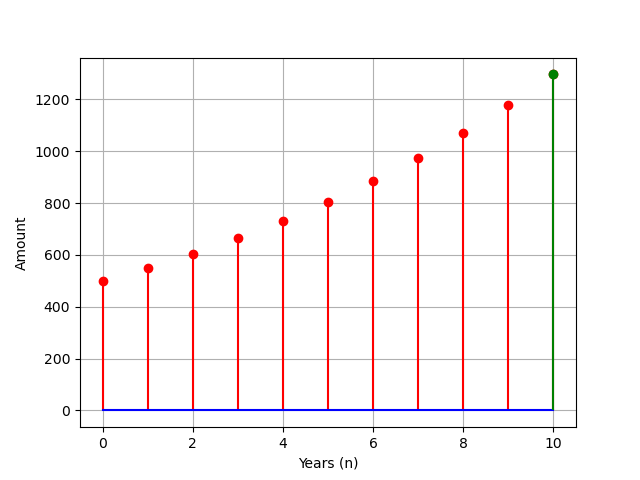
\includegraphics[width = 8cm]{ncert-maths/11/9/3/31/figs/Fig1.png}
		     \caption{Plot of $x(n) = 500(1.1)^n$}
		         \label{fig:enter-label.11.9.3.31}
 \end{figure}
